\documentclass[a4paper]{article}

\usepackage{numprint}
\usepackage{nameref}
\usepackage{float}
\usepackage{url}
\usepackage{graphicx}	% For figure environment
\usepackage{epstopdf}
\usepackage[center]{subfigure}
\usepackage{amssymb}	% For mathematical figures like \mathbb{R}
\usepackage{amsmath}
\usepackage{framed}
\usepackage{tikz}
\usetikzlibrary{mindmap,trees}
\usepackage{pdflscape}
\usepackage[a4paper]{geometry}
\usepackage{subfiles}
\usepackage{listings}
\usepackage{color}

\definecolor{dkgreen}{rgb}{0,0.6,0}
\definecolor{gray}{rgb}{0.5,0.5,0.5}
\usepackage{array}
\usepackage{booktabs}% http://ctan.org/pkg/booktabs
\usepackage{xparse}% http://ctan.org/pkg/xparse
% Rotation: \rot[<angle>][<width>]{<stuff>}
\NewDocumentCommand{\rot}{O{45} O{1em} m}{\makebox[#2][l]{\rotatebox{#1}{#3}}}%
\definecolor{mauve}{rgb}{0.58,0,0.82}

\lstset{frame=tb,
  language=Java,
  aboveskip=3mm,
  belowskip=3mm,
  showstringspaces=false,
  columns=flexible,
  basicstyle={\small\ttfamily},
  numbers=none,
  numberstyle=\tiny\color{gray},
  keywordstyle=\color{blue},
  commentstyle=\color{dkgreen},
  stringstyle=\color{mauve},
  breaklines=true,
  breakatwhitespace=true
  tabsize=3
}


\title{Advanced Systems Lab - Milestone II} 
\author{Matthias Ganz (ganzm@ethz.ch)} 
\date{\today} 


\begin{document}

\maketitle

\pagebreak

\tableofcontents

\pagebreak

\begin{abstract}

This document describes an analytical model of the message queuing system which was build during Milestone I. Analytical studies are presented and compared with the results obtained before.


\end{abstract}

\pagebreak

%% ----------------------------------------------
% Section - The System
%% ----------------------------------------------
\section{The System}

This chapter should briefly show the most important components of the System Under Test (SUT). The curious reader is referred to the document Milestone I. In depth information about the technical details are stated there.


% ------------------------------------------------
% Figure 

\begin{figure}[H]
	\begin{center}
    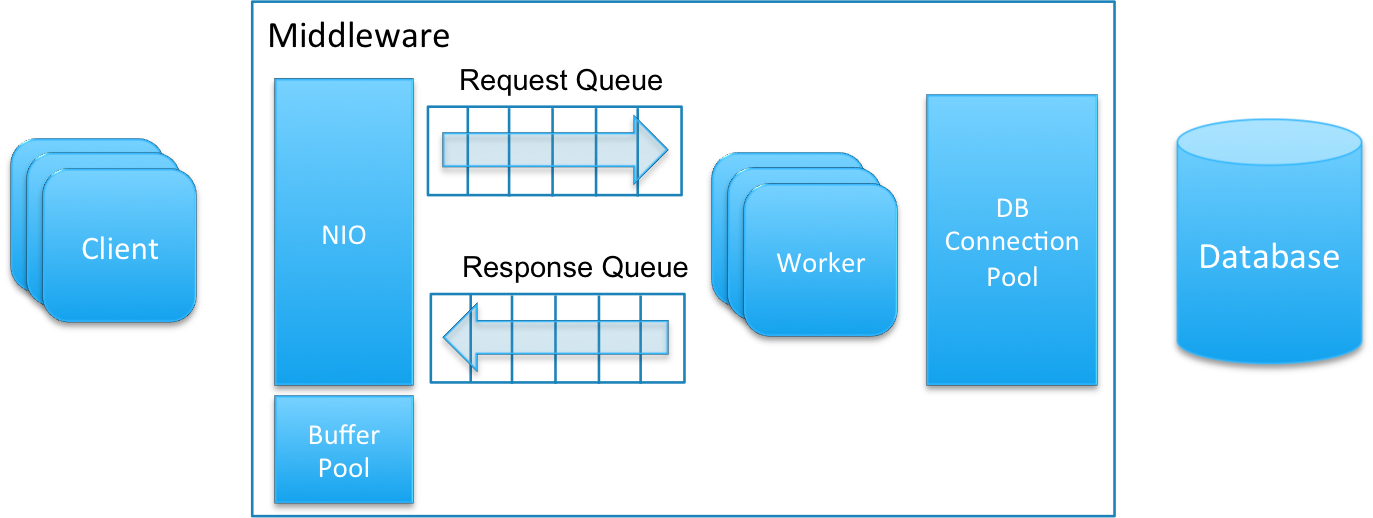
\includegraphics[scale=0.4]{../drawings/broker-threading.png}
  \end{center}
  \caption{System Under Test}
  \label{fig:sut}
\end{figure}

%% ----------------------------------------------

Requests from clients are read and pushed to Request Queue. This Queue is processed by a fixed numer of worker threads which utilize pooled database connections to generate an appropriate response. Theses responses are put back into the response queue which is processed by the networking interface.


%% ----------------------------------------------
% Section System Model
%% ----------------------------------------------
\section{Model of the System}

\subsection{Modelling a closed system}
Due to the nature of the tests performed during Milestone I the system should be modeled as a closed queuing system. Each experiment was performed with a fixed number of clients. Each client is issuing at max one concurrent request. Therefore the number of messages in the system never exceed the number of clients.


% ------------------------------------------------
% Figure 

\begin{figure}[H]
	\begin{center}
    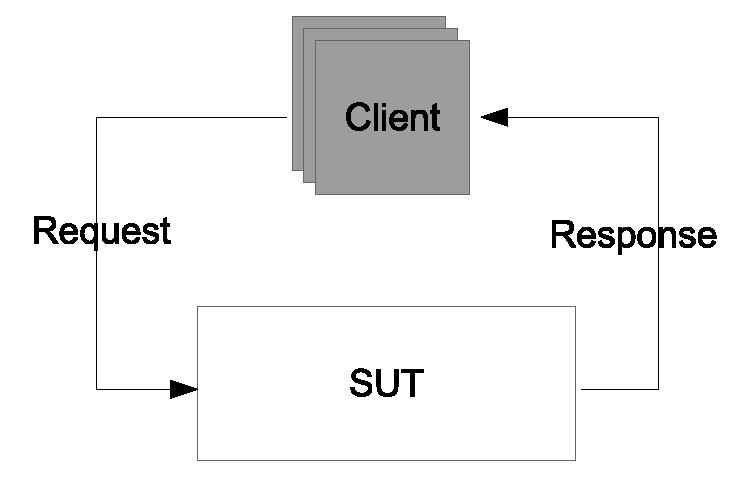
\includegraphics[scale=0.4]{../drawings-ms2/sut.eps}
  \end{center}
  \caption{Closed System}
  \label{fig:closedsystem}
\end{figure}

%% ----------------------------------------------



\subsection{Kendall's Notation}
In this chapter we look at the system as a black box. To describe it \textit{Kendall's Notation} is used. The 6 characteristic parameters A/S/m/B/K/SD are defined as followed.

\subsubsection{(A) Arrival Process}

The interarrivaltime is assumed to be exponentially distributed. This can be shown from figure \ref{fig:interarrivaltime}. Therefore parameter a) is M (Markovian)


% ------------------------------------------------
% Figure 

\begin{figure}[H]
	\begin{center}
    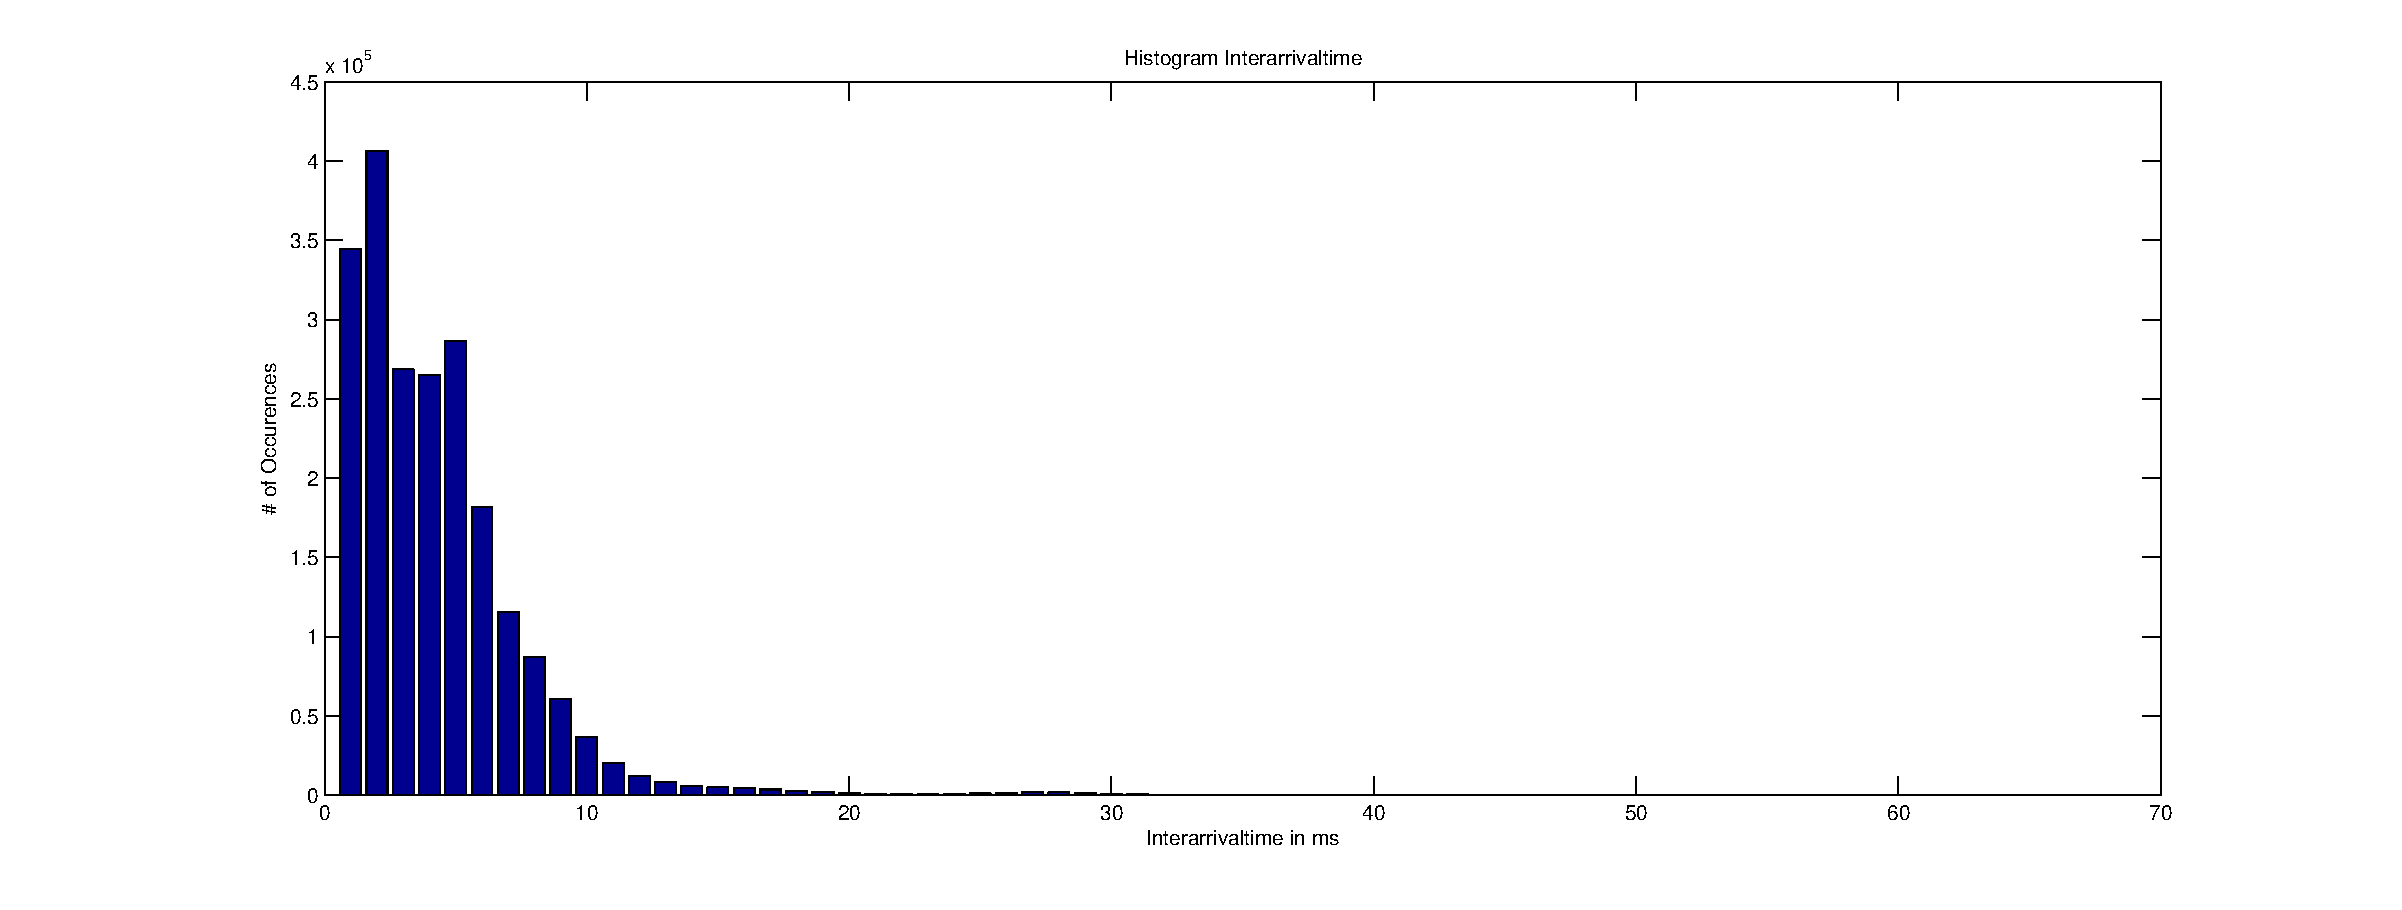
\includegraphics[scale=0.5]{../plots-ms2-mg/interarrivaltime.eps}
  \end{center}
  \caption{Histogram Interarrivaltime}
  \label{fig:interarrivaltime}
\end{figure}

%% ----------------------------------------------


\subsubsection{(S) Service Time Distribution }

Again it is assumed that the service time distribution is memoryless exponentially distributed. TODO see figure.

\subsubsection{(m) Number of Servers}

This parameter is determine by the number of middleware instances running.

\subsubsection{(B) Buffer - System Capacity }


\subsubsection{(K) Population Size}


\subsubsection{(SD) Service Disciplin}
Because the whole messaging system consists of queues  First Come First Server (FCFS) service disciplin is assumed for our system model.


\section{Refined System Model}

Modeling the system as a black box is not very accurate. To be able to do a more distinct analysis and to identify bottle neck components a queueing ...

\subsection{Service Centers}

From figure \ref{fig:sut} on can derive the following components of the system model.

\subsubsection{Network Receive}
The first queue where clients issue requests is the networking part of the middle ware. The queue size of this not too clear \\

\begin{tabular}{|l|c|}
\hline 
Queue Size & Number of clients \\ 
\hline 
Service Node Count & 1 \\ 
\hline 
\end{tabular} 

\subsubsection{Request Queue}
This node represents the request queue and the worker threads attached to it.\\

\begin{tabular}{|l|c|}
\hline 
Queue Size & Corresponds to Request Queue size (default 50)\\ 
\hline 
Service Node Count & Corresponds to \# of worker thread \\ 
\hline 
\end{tabular} 

\subsubsection{Database}
This node represents the database. For the experiment an Amazon medium instance with two ECU's (EC2 Compute Units)

\begin{tabular}{|l|c|}
\hline 
Queue Size & Corresponds to Request Queue size (default 50)\\ 
\hline 
Service Node Count & Corresponds to the total number of database connections \\ 
\hline 
\end{tabular} 


\subsubsection{Network Send}




\section{Memos}

- create a single queue system with the 

- hierarchical decomposition

- decompose into smaller network

\section{Refined Model of the System}


\section{Mean-Value Analysis}



%% ----------------------------------------------
% Section MEMOS
%% ----------------------------------------------
\section{Memos}

open or closed system
- do we have an open or a closed system? It's closed!

- use bullshit word "service center"

- build alanytical queuing model of the whole system
  - parameters
- build alanytical queuing model for each part of the system
  - parameters
- explain where data matches the model and where not

- interactive response time law, not applicable because of client implementation

analytical model, 


- network of queues
  - not too fine, abstract away threads
  
  
- explain why the model matches reality (or not)


- siehe buch seite 1078 für Anregungen was man so machen müsste


\end{document}

